\section[Advice]{General advice}

\subsection{}

\begin{frame}
    \frametitle{Hardware}
    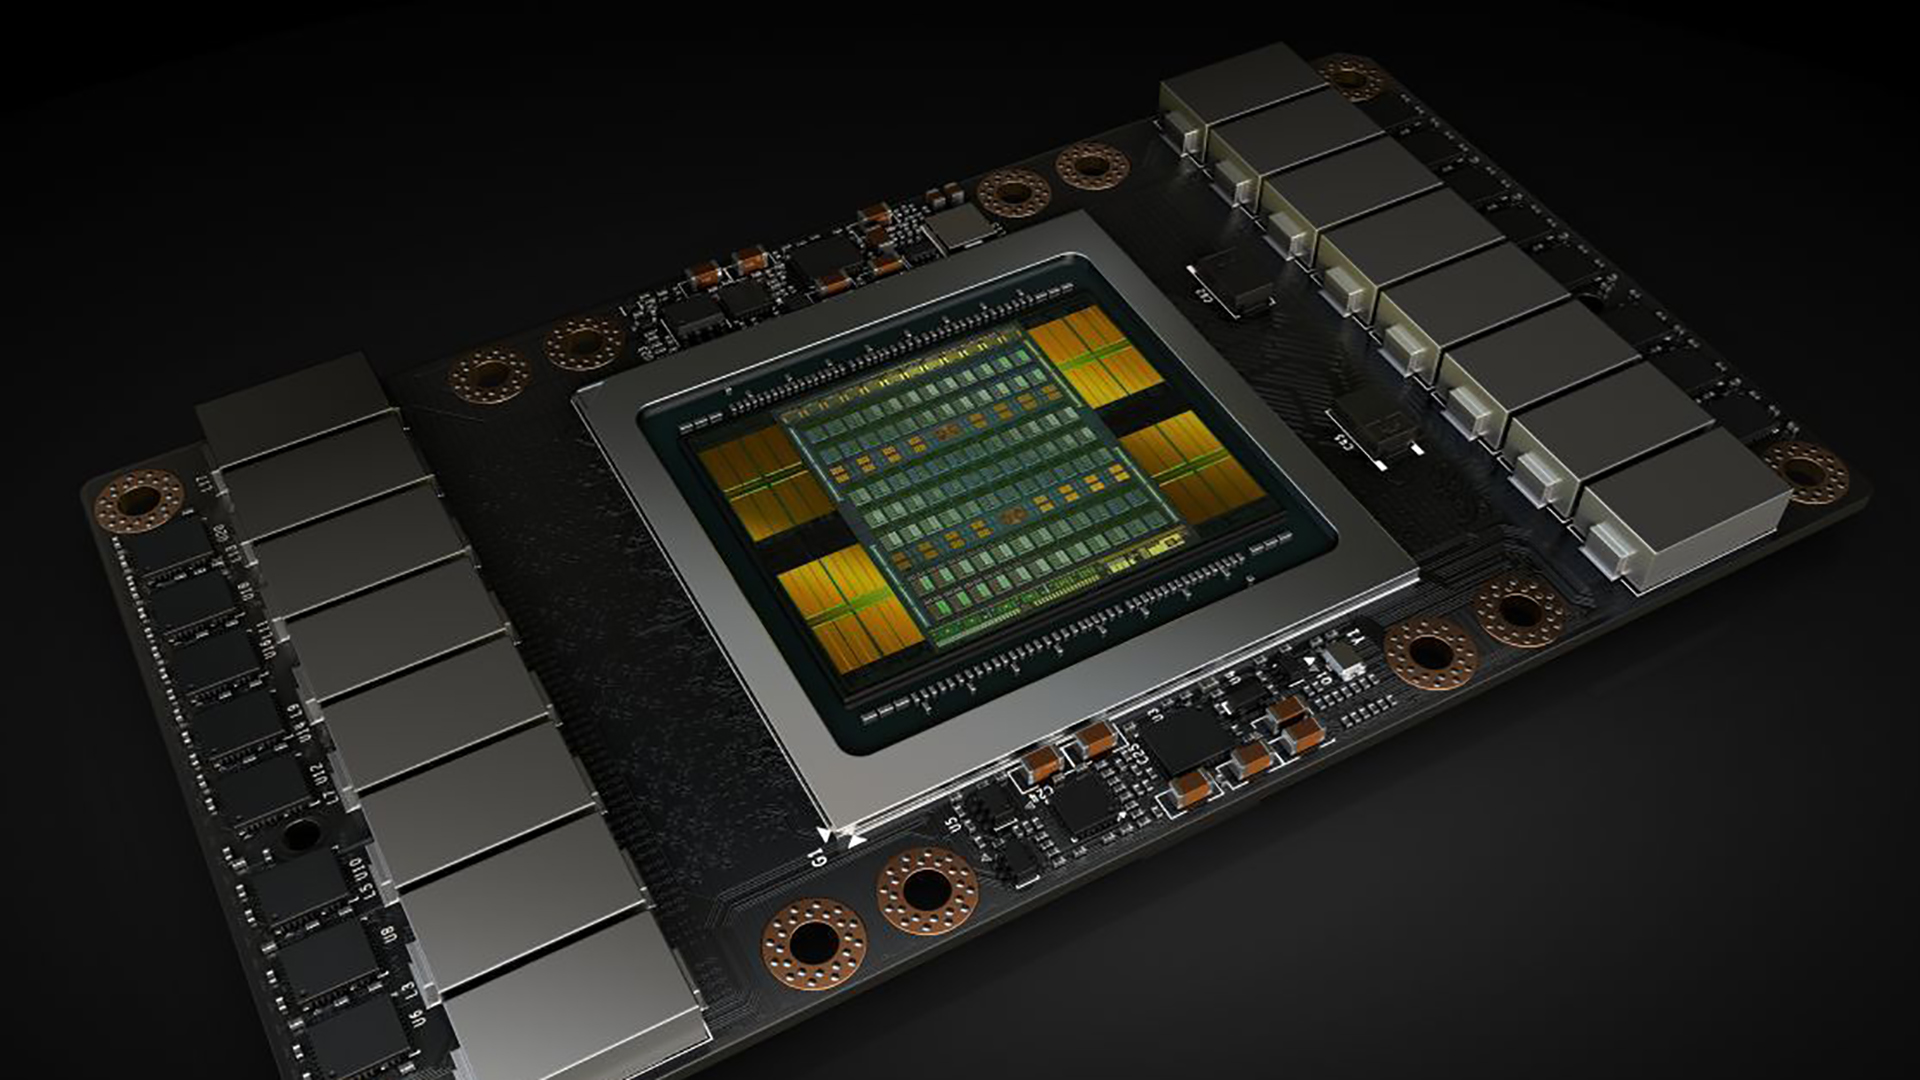
\includegraphics[width=0.48\textwidth]{volta}
    \hfill
    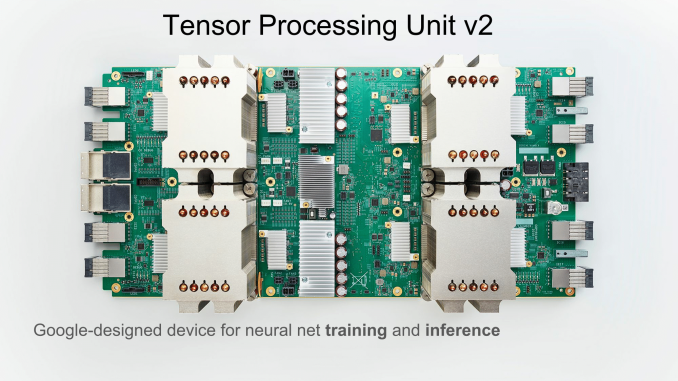
\includegraphics[width=0.48\textwidth]{tpu}

    \begin{itemize}[<+->]
        \item \alert{Use GPUs.}
        The bulk of forward and backprop is matrix--vector multiplies; common for GPUs to be $\O(10 \text{--} 100)\times$ faster than CPUs
        \item \alert{Use GPUs built for NNs.}
        NVIDIA Volta and Google tensor processing unit (TPU) are built from ground-up to be lightning fast for NNs (e.g., 16-bit multiply-add for 32-bit result)
        \item \alert{Use mini-batch sizes and widths that are integer powers of 2.}
        Not a hard rule, but GPUs tend to more efficient this way
        \item \alert{Use 32-bit floats.}
        Neural networks are not turbulence simulations; no tangible benefit to 64-bit doubles
    \end{itemize}
\end{frame}

\begin{frame}
    \frametitle{Software}
    \begin{itemize}
        \item $\exists$ many NN platforms; unclear which will win out in the end.
        \item Most popular now: Keras, TensorFlow, PyTorch
        \begin{itemize}
            \item TensorFlow seems to be winning, but list changes rapidly
        \end{itemize}
        \pause
        \item How do they compare in my opinion?
    \end{itemize}

    \begin{center}
        \begin{tikzpicture}
    \def\pos{0}
    \scale{difficult}{easy}
    \entry{TF}{-3}
    \entry{PT}{-1}
    \entry{K}{3}

    \def\pos{-1.5}
    \scale{limited \\ capability}{flexible}
    \entry{K}{-3}
    \entry{TF}{1.7}
    \entry{PT}{3}

    \def\pos{-3}
    \scale{limited \\ docs}{excellent \\ docs}
    \entry{K}{-1.2}
    \entry{TF}{1.5}
    \entry{PT}{3}

    \def\pos{-4.5}
    \scale{small \\ user base}{large \\ user base}
    \entry{PT}{-1.5}
    \entry{K}{1}
    \entry{TF}{3}
\end{tikzpicture}
%%% Local Variables:
%%% mode: latex
%%% TeX-master: "../nn"
%%% End:

    \end{center}
\end{frame}

\begin{frame}
    \frametitle{Neural network architecture}
    \begin{itemize}[<+->]
        \item \alert{Use CNNs for spatial data \& RNNs for temporal data.}
        \item \alert{Start with architectures that are too small.}
        NNs take a long time to train; make problems show up immediately.
        \item \alert{Scale up architectures until they overfit.}
        Check the relation between NN size and validation loss.
        Back off on size if validation loss increases.
        \item \alert{Use pretraining.}
        If applicable, borrow NN architecture from pre-existing model (e.g., ResNet), and initialize parameters to trained values from different task.
        \item \alert{Use dropout.}
        They are one of the best regularizers.
        \item \alert{Aim for $\text{\# parameters} \le \text{\# data}$.}
        Helps prevent overfitting.
        \item \alert{Set layer $i$ to be \sfrac{1}{2}--\sfrac{3}{4} the width of layer $i - 1$.}
        Layers closer to the input have greater expressive power.
        \item \alert{Beware of excessive depth.}
        They make NNs much harder to train and can cause overfitting.
    \end{itemize}
\end{frame}

\begin{frame}
    \frametitle{End-to-end machine learning}

    \begin{block}{}
        \alert{End-to-end}: give the model input \& output data, but don't tell it how to get from inputs to outputs.
        Let the model figure it out.
    \end{block}

    \begin{center}
        \begin{tikzpicture}[node distance=1.5cm]
    \node (audio) [draw, block, fill=yellow!20, align=center] {speech \\ audio};
    \node (box) [draw, block, fill=black!20, minimum height=1.3cm, minimum width=1.3cm, align=center, right=of audio] {black box};
    \node (text) [draw, block, fill=yellow!20, right=of box] {text};

    \draw [path] (audio) -- (box);
    \draw [path] (box) -- (text);
\end{tikzpicture}

%%% Local Variables:
%%% mode: latex
%%% TeX-master: "../nn"
%%% End:

    \end{center}
    \pause

    \begin{block}{}
        Alternative: define intermediate variables; train models from inputs to intermediate variables to outputs
    \end{block}

    \begin{center}
        \begin{tikzpicture}[node distance=4.4mm]
    \node (audio) [draw, block, fill=yellow!20, align=center] {speech \\ audio};
    \node (box 0) [draw, block, fill=black!20, right=of audio] {FFT};
    \node (spectrum) [draw, block, fill=blue!20, right=of box 0] {spectrogram};
    \node (box 1) [draw, block, fill=black!20, align=center, right=of spectrum] {black \\ box};
    \node (phonemes) [draw, block, fill=blue!20, right=of box 1] {phonemes};
    \node (box 2) [draw, block, fill=black!20, align=center, right=of phonemes] {black \\ box};
    \node (text) [draw, block, fill=yellow!20, right=of box 2] {text};

    \draw [path] (audio) -- (box 0);
    \draw [path] (box 0) -- (spectrum);
    \draw [path] (spectrum) -- (box 1);
    \draw [path] (box 1) -- (phonemes);
    \draw [path] (phonemes) -- (box 2);
    \draw [path] (box 2) -- (text);
\end{tikzpicture}

%%% Local Variables:
%%% mode: latex
%%% TeX-master: "../nn"
%%% End:

    \end{center}
    \pause

    \begin{itemize}
        \item End-to-end can learn very complex input--output relations\ldots
        \item But requires enormous data and very powerful models/optimizers
        \item Often best not to start with end-to-end
    \end{itemize}
\end{frame}

\begin{frame}
    \frametitle{Data}

    \begin{itemize}
        \item<+-> \alert{Normalize the data, or use batch normalization.}
        NNs learn better if inputs look standard normal and uncorrelated.
        \item<+-> \alert{Don't extrapolate.}
        Models are meaningless outside their domain of training.
        \begin{itemize}
            \item E.g., sigmoid/ReLU activations have 0th/1st order extrapolation
        \end{itemize}
    \end{itemize}

    \begin{columns}
        \begin{column}{0.4\textwidth}
            \centering
            \footnotesize

            \visible<+->{
                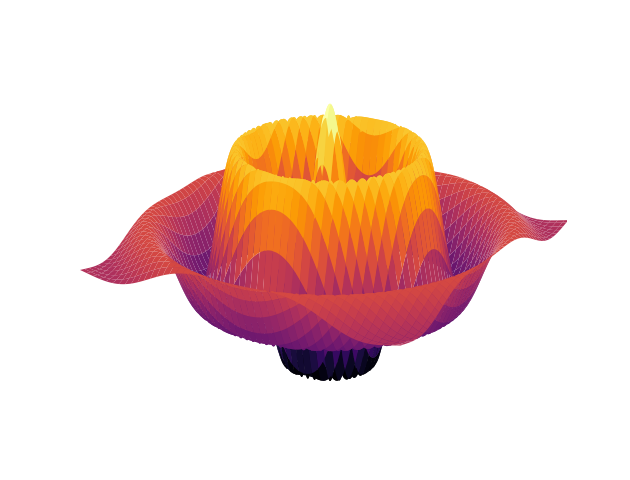
\includegraphics[width=1.5in]{ripple} \\
                ground truth, $[-12, 12] \times [-12, 12]$
            }
            \visible<+->{
                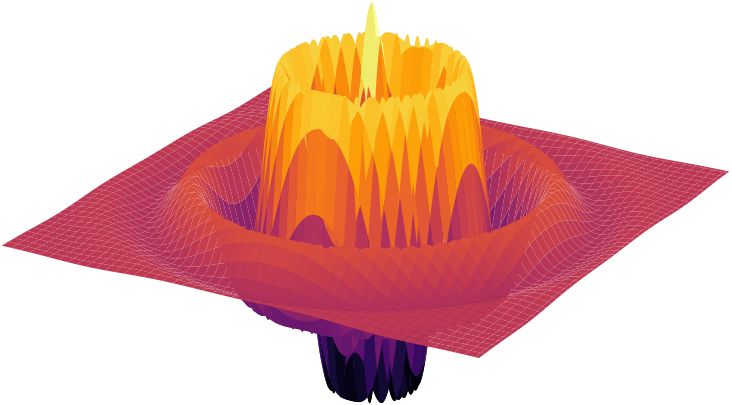
\includegraphics[width=1.5in]{extended_ripple} \\
                ground truth, $[-18, 18] \times [-18, 18]$
            }
        \end{column}

        \begin{column}{0.6\textwidth}
            \centering
            \footnotesize

            \setcounter{beamerpauses}{3}
            \visible<+->{
                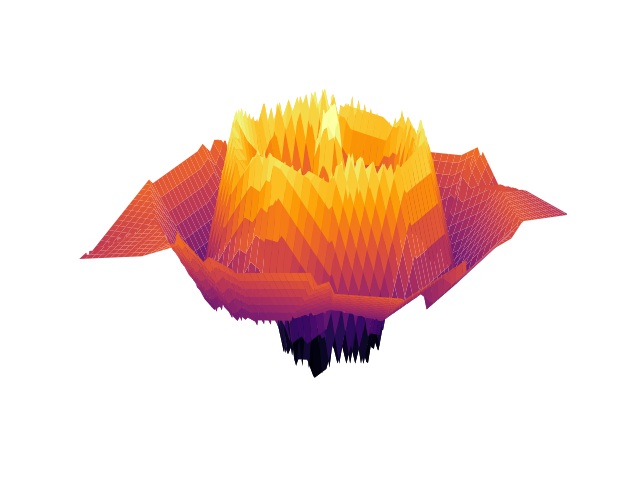
\includegraphics[width=1.5in]{ripple_2layer} \\
                17--8 neurons, $[-12, 12] \times [-12, 12]$
            }
            \visible<+->{
                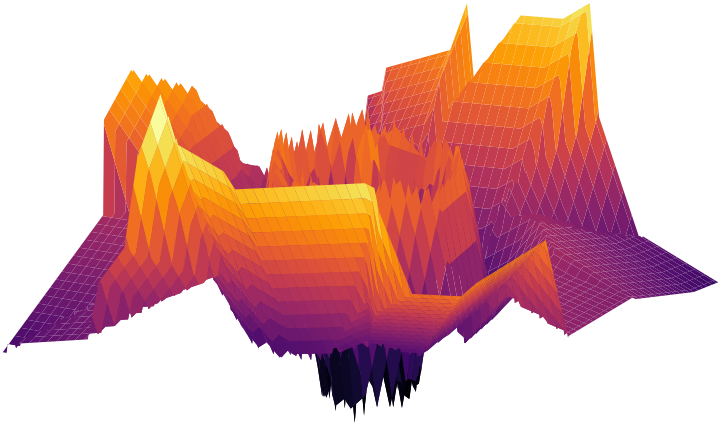
\includegraphics[width=1.5in]{extrapolated_ripple} \\
                above model extrapolated to $[-18, 18] \times [-18, 18]$
            }
        \end{column}
    \end{columns}
\end{frame}

\begin{frame}
    \frametitle{Engaging with the scientific community}

    \begin{itemize}
        \item<+-> \alert{Stay on top of recent conferences and arXiv papers.}
        Papers seem to become obsolete after 2 years.
        \item<+-> \alert{Be aware of \emph{interpretability} criticisms, but do not fear them.}
        \begin{itemize}[<+->]
            \item Main reason physicists reject machine learning: \\[1ex]

            \emph{``So you made a model with 1,000,000,000 parameters, and you fit the data, but you haven't a clue what any of those parameters actually means, or why your model does what it does.''} \\[1ex]

            \ldots or something like that
            \item ML community divided on whether interpretability is important
            \item But don't ignore the results: \emph{ML works}, whether you understand its inner workings or not
            \item<.-> (I drive a car everyday, and I understand its behavior, but I have no idea how it works)
        \end{itemize}
    \end{itemize}
\end{frame}

%%% Local Variables:
%%% mode: latex
%%% TeX-master: "../nn"
%%% End:
